\documentclass{article}

\usepackage[T1]{fontenc}
\usepackage{amsmath}
\usepackage{amssymb}
\usepackage{graphicx}
\usepackage{titling}
\usepackage{ragged2e}
\usepackage{lipsum}
\usepackage{booktabs}
\usepackage{fancyvrb}
\usepackage[hidelinks]{hyperref}
\usepackage[a4paper,left=0.75in,right=0.75in,top=1in,bottom=1in,footskip=0.5in]{geometry}

\pretitle{\vspace{1in}\hrulefill\par}
\posttitle{\par\hrulefill}

\title{\begin{center}\Huge COMP2432\\
    G06 Group Project Reoprt\end{center}}
\date{}
\author{}

\begin{document}
    \begin{titlepage}
        \maketitle
        \begin{center}
            \huge Room Booking Manager
            \vfill
            \begin{table}[!htbp]
                \centering
                \huge
                \begin{tabular}{ll}
                    19081789D\hspace{0.25in}&MAN, Furui \\
                    19078543D\hspace{0.25in}&WANG, Meng \\
                    18080998D\hspace{0.25in}&WU, Junyu  \\
                    19079008D\hspace{0.25in}&XING, Shiji\\
                \end{tabular}
            \end{table}
            \vspace{0.5in}
            \thispagestyle{empty}
        \end{center}
    \end{titlepage}
    \cleardoublepage
    \tableofcontents
    \thispagestyle{empty}
    \cleardoublepage
    \setcounter{page}{1}
    \section{Introdoction}
        \paragraph{}
        The project aims to utilize the knowledge covered in COMP2432 Operating Systems
        and put them into practice to get a further understanding and improvement. This
        works out by implementing a facility management system for a company, which
        would make advantage of all kinds of scheduling skills and abstractions covered
        in the lecture, along with the use of multi-process programming and inter-process
        communication. 
    \cleardoublepage
    \section{Scope}
        \paragraph{}
        Multi-Process Programming and Inter-process Communication: pipe() and fork(); 
        \paragraph{}
        CPU Scheduling: FCFS and PR 
        \paragraph{}
        Memory Allocation: MFT
        \paragraph{}
        Synchronization: Program-Monitored Synchronization 
    \cleardoublepage
    \section{Concept}
        \subsection{FCFS Scheduling}
            \paragraph{}
                FCFS scheduling is indeed taking the arriving time of the request as the
                priority. It is very easy to implement this algorithm, as long as the
                order of the request array is the same order as input, which is very
                natural. One thing to note that to keep the order of request array the
                same as input order, Input Module must be single-threaded. 
        \subsection{PRIO Scheduling}
            \paragraph{}
            It is already mentioned that FCFS is a special case of PRIO scheduling where
            the priority is the arriving time. Now that a priority is appended with the
            request, all it needs is to sort the request array by priority, then call
            FCFS scheduling to implement PRIO scheduling. This reuses the code and
            decrease the complexity of the program. 
    \cleardoublepage
    \section{Design of opti}

    \cleardoublepage
    \section{Program Structure}
        \subsection{Class Design}
            \begin{figure}[!htbp]
                \centering
                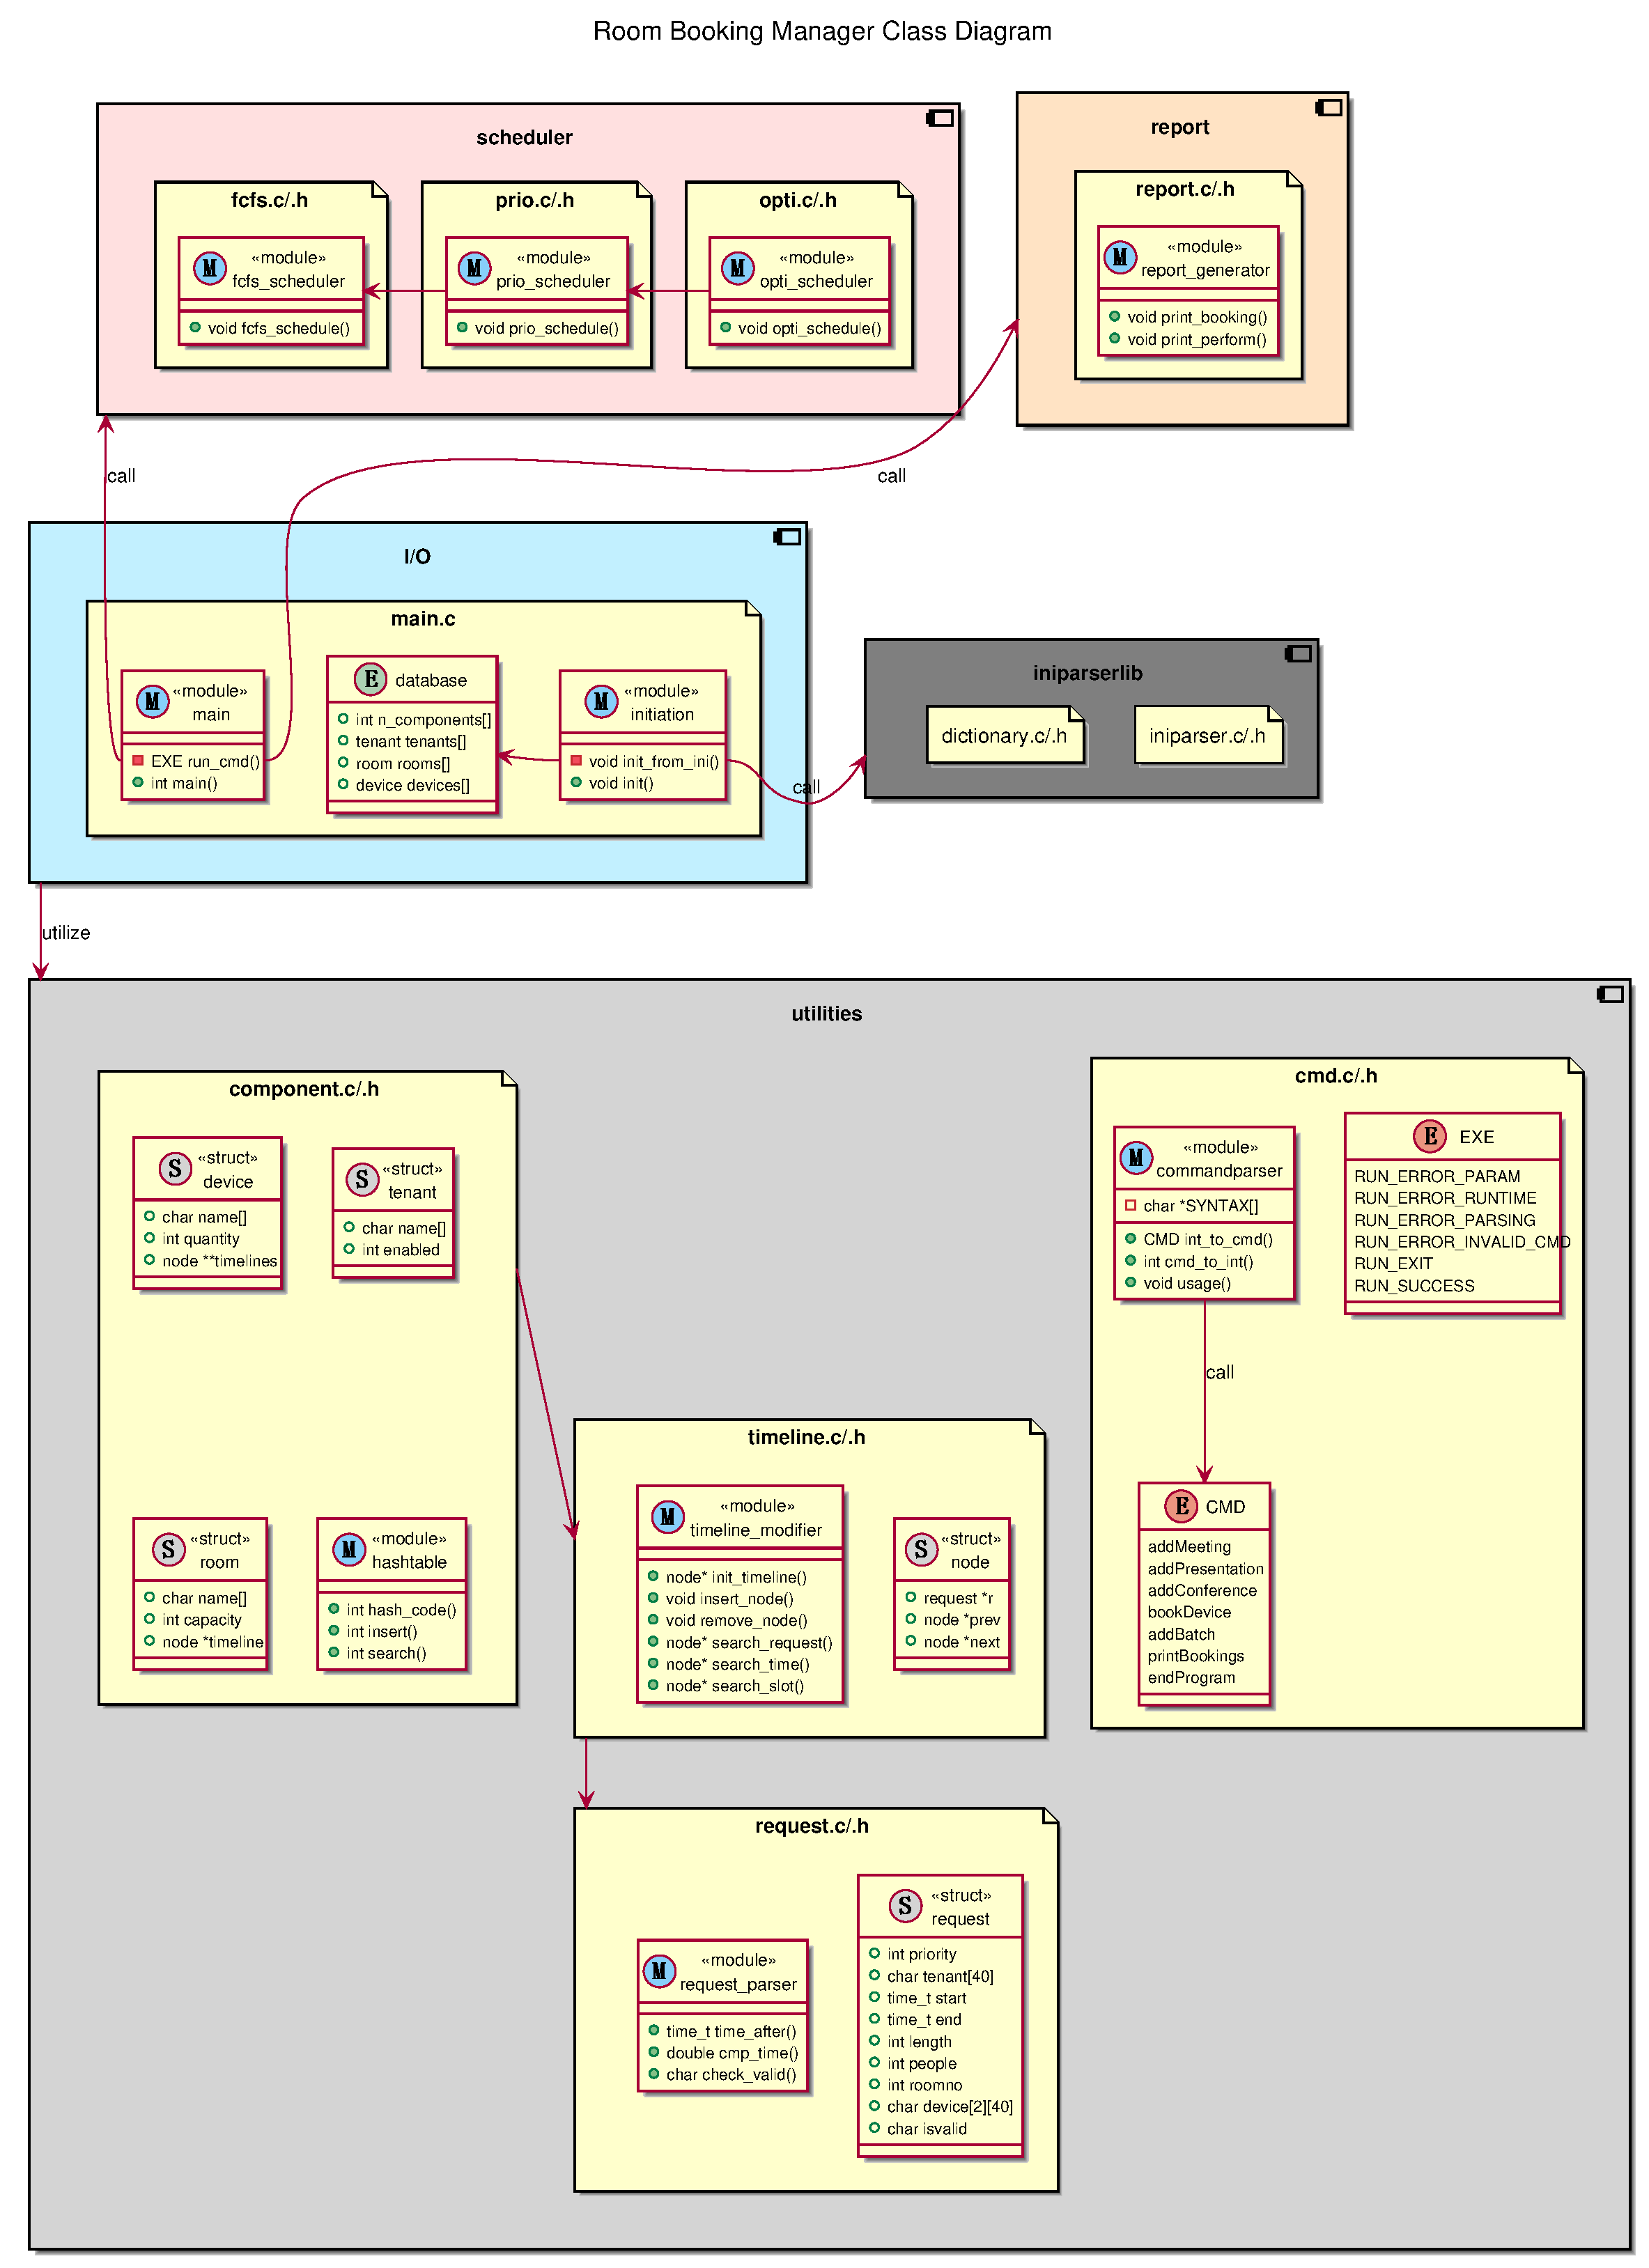
\includegraphics[scale=0.4]{./img/class_diagram.eps}
                \caption{Overall class design diagram of Room Booking Manager}
            \end{figure}
        \subsection{Sequence Design}
            \begin{figure}[!htbp]
                \centering
                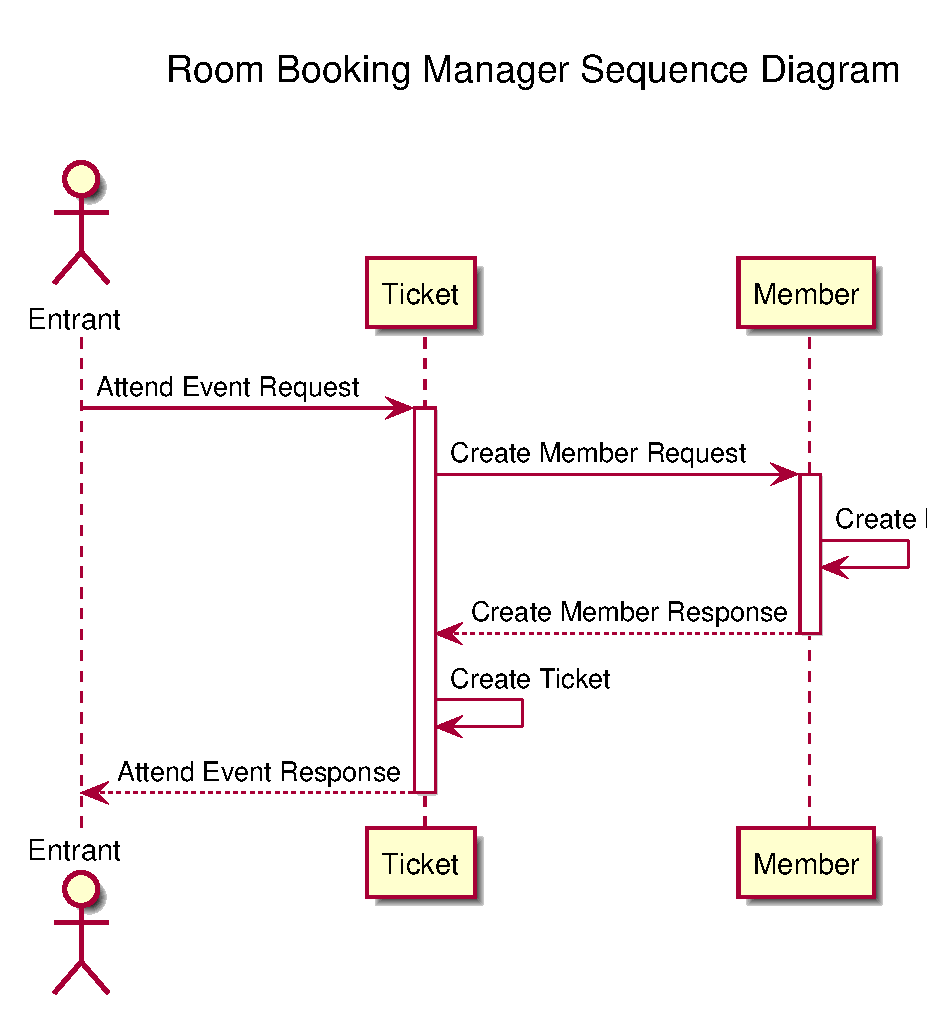
\includegraphics[scale=0.5]{./img/sequence_diagram.eps}
                \caption{Overall sequence design diagram of Room Booking Manager}
            \end{figure}
        \subsection{Activity Design}
            \begin{figure}[!htbp]
                \centering
                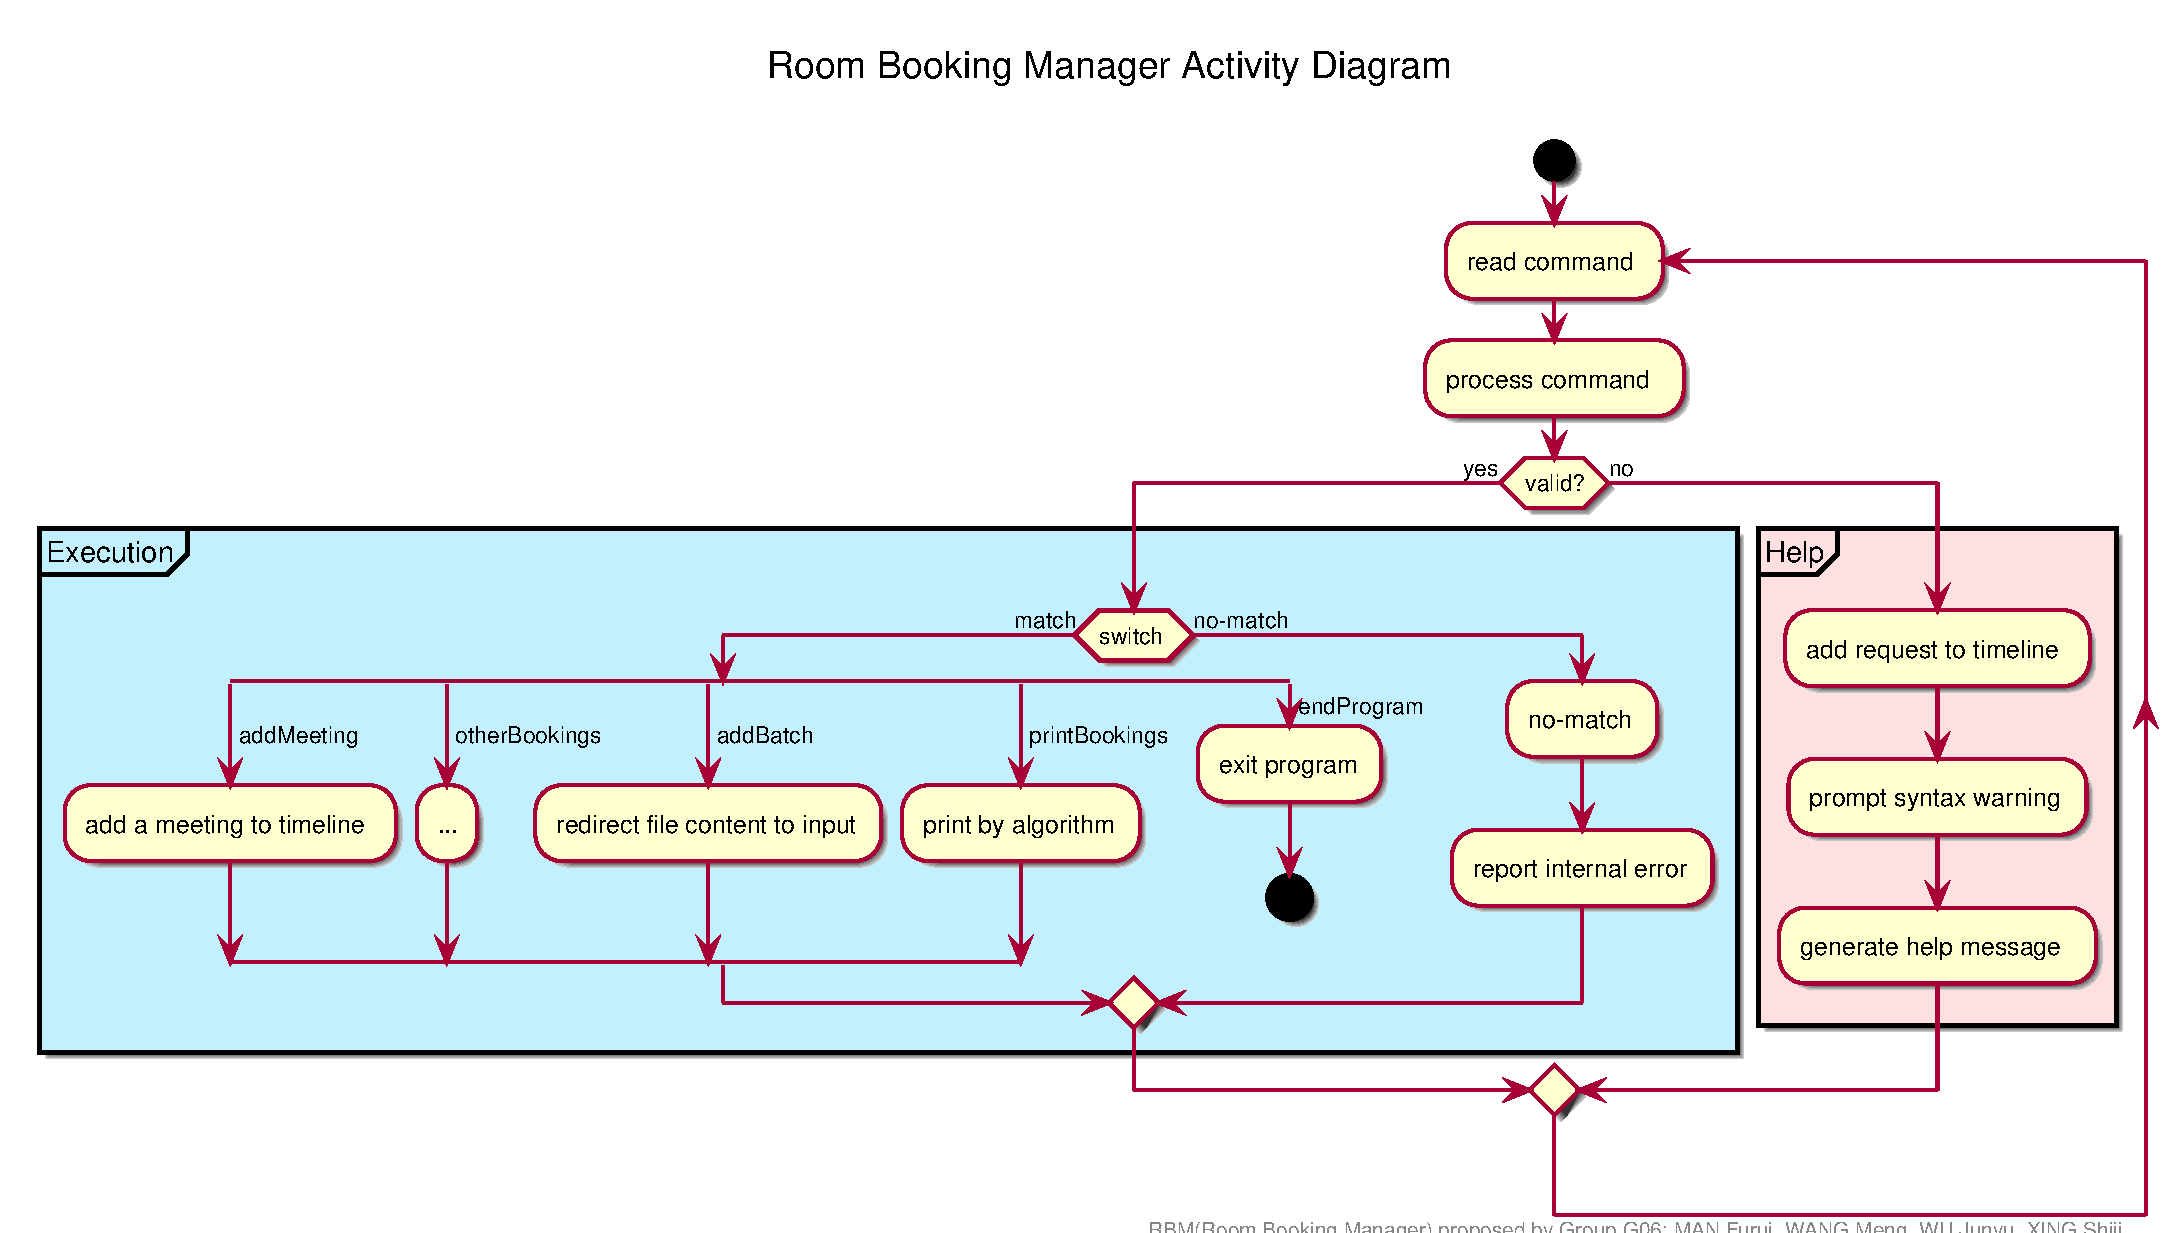
\includegraphics[scale=0.45]{./img/activity_diagram.eps}
                \caption{Overall activity design diagram of Room Booking Manager}
            \end{figure}

    \cleardoublepage
    \section{Testing Cases}
        \paragraph{}
        This is the brief version, which demonstrates the valid and invalid tests for addMeeting instruction only.
        \paragraph{}
        Tests for other instructions are similar and therefore not included. Syntax of other instructions varies in
        number of the parameters. Help message on syntax is available once an input error is detected.
        \paragraph{}
        Refer to the appendix for the full version. 

        \paragraph{valid tests}
        \paragraph{}
        Valid syntax for addMeeting instruction should be:
        \begin{Verbatim}[gobble=8]
            addMeeting -tenant YYYY-MM-DD hh:mm n.n [d1 d2]; 
        \end{Verbatim}
        \paragraph{}
        Below are some samples which conforms the above syntax:
        \begin{Verbatim}[gobble=8]
            addMeeting -tenant_A 2021-05-10 21:50 1.50 5 projector_2K screen_100;
            addMeeting -tenant_A 2021-05-11 18:20 0.30 5;
            addMeeting -tenant_A 2021-05-11 4:10 0.0 5;
        \end{Verbatim}
        
        
        \paragraph{invalid tests}
        \paragraph{}
        Invalid instructions of addMeeting are either:
        
        \begin{itemize}
        \item Syntax invalid: (including command invalid, tenant invalid, date invalid, hour and minute invalid,
        duration invalid, number of people invalid, device invalid); or
        \end{itemize}
        
        \begin{Verbatim}[gobble=8]
            command_invalid and parameters does not matter;
            addMeeting -tenant_invalid 2021-05-10 1:30 0.50 5 projector_2K screen_100;
            addMeeting -tenant_A date-in-valid 1:30 0.50 5 projector_2K screen_100;
            addMeeting -tenant_B 2021-05-10 hhmm:invalid 1.50 5 webcam_FHD monitor_75;
            addMeeting -tenant_C 2021-05-10 18:30 duration.invalid 5 webcam_FHD monitor_50;
            addMeeting -tenant_D 2021-05-10 10:40 0.0 peopleinvalid projector_2K screen_150;
            addMeeting -tenant_D 2021-05-16 3:10 1.10 5 device_invalid monitor_50;
        \end{Verbatim}
        \begin{itemize}
        \item Device pairing error (devices must be in pairs).
        \end{itemize}
        \begin{Verbatim}[gobble=8]
            addMeeting -tenant_E 2021-05-10 22:20 0.50 5 projector_4K monitor_50; 
            addMeeting -tenant_E 2021-05-10 22:20 0.50 5 projector_4K; 
        \end{Verbatim}
        

    \cleardoublepage
    \section{Performance analysis}

    \cleardoublepage
    \section{Program Setup \& Analysis}
        \subsection{Program Setup}
            \paragraph{Step 0 Clone repo(optional)}
            \paragraph{}
                Clone the repo from Github if there is no local copy.
                \begin{Verbatim}[gobble=8]
                    git clone https://github.com/toolsmax0/COMP2432_RBM.git
                \end{Verbatim}
            \paragraph{Step 1 Compilation}
            \paragraph{}
                \texttt{cd} to the project's root directory and execute \texttt{build.sh} script.
            \paragraph{}
                The program have dependency upon \texttt{gcc 4.0+} and \texttt{linux 3.0+}.
                \begin{Verbatim}[gobble=8]
                    cd COMP2432_RBM
                    sh build.sh
                \end{Verbatim}
            \paragraph{Step 2 Costomization(optional)}
            \paragraph{}
                To modify the component settings (i.e. tenants, rooms, devices),
                modify \texttt{RBM.ini} file according to its syntax.
            \paragraph{Step 3 Execution}
            \paragraph{}
                To execute the program, run the following command.
                \begin{Verbatim}[gobble=8]
                    ./out/RBM
                \end{Verbatim}

        \subsection{Progarm Analysis}
            
    \cleardoublepage
    \section{Appendix}
        \subsection{Source Code}
            \paragraph{}
                All source files are located under \texttt{./src/} directory. Please \texttt{cd}
                to corresponding directory for reference.
        \subsection{Test Data}
            \paragraph{}
                All test data are generated with \texttt{generator.py} under \texttt{./test/}
                directory. Sufficient amount of test cases are generated via this generator
                and stored into \texttt{*.dat} files.
            \paragraph{}
                All files of test data are located under \texttt{./test/} directory. Please
                \texttt{cd} to corresponding directory for reference.
            \paragraph{}
                Files marked with \texttt{*\_invalid.dat} are invalid tests for specific command
                types. The rest of files are for valid tests.
        \subsection{Test Results}
            \paragraph{}
                Warnings should be generated for each invalid case, while not for valid cases. 
            \paragraph{}
                The descriptions of valid/invalid tests have been clearly stated under
                \textbf{9.2 Test Data}.
        \subsection{Sample Output}
            \paragraph{}
                Output of test files are stored in \texttt{sample\_output\_*.txt} file under
                \texttt{./test/} directory with algorithm applied. Please refer to the
                corresponding file for reference.
                
\end{document}